Nuclear forensics comprises a large part of an investigation into a nuclear
incident, such as interdicted nuclear material or the detonation of a weapon
containing radioactive components.  The forensics portion of the investigation
encompasses both the analysis of nuclear material and/or related paraphrenalia
as well as the interpretation of these results to establish nuclear material
provenance. The former has many technical aspects, relying on a range of
nuclear science and chemistry.  The latter involves intelligence and political
considerations of the material analyses for attribution. This review will only
consider the technical portion of the nuclear forensics workflow.

First discussed are the types of forensic investigations in Section
\ref{sec:types}, followed by an introduction to inverse problem theory in
Section \ref{sec:inverse} as a way to evaluate the results of forensic methods. 

\subsection{Types of Nuclear Forensics Investigations}
\label{sec:types}

The technical programs researching improvements to the \gls{US}'s nuclear
forensics capabilities are split between the type of material being
investigated. The analysis of irradiated debris from a weapon has different
collection and measurement requirements than a mass of \gls{SNM}. This
separates the field into post-detonation and pre-detonation nuclear forensics.
While both are discussed below in Sections \ref{sec:postdet} and
\ref{sec:predet}, respectively, there is more focus on pre-detonation topics
since this work is based on \gls{SNF}.

\subsubsection{Post-Detonation}
\label{sec:postdet}

Post-detonation nuclear forensics requires a diverse set of measurements to
obtain the following information: identification of nuclear material,
reconstruction of the weapon device design, and reactor parameters for nuclear
material provenance. This could apply to an improvised nuclear device or a
nuclear bomb.  In conjunction with the measurements and characterization are a
large array of logistical concerns, including recovery efforts, personnel
safety, and material collection cataloging and transportation.

In the case of a full explosion using fissile material, the collection of
materials and debris occurs as quickly as possible.  It can be in the crater
created by the explosion, further away from the center in the fallout, and in
the atmosphere above or downwind from the detonation. These are collected by
finding glass-like material near the epicenter, debris swipes in the fallout
region, and advanced particle collection in the atmosphere via an airplane,
respectively.  While the epicenter cannot be reached for some time, the debris
and atmosphere measurements of radioactive material can provide the yield of
the weapon and whether it was made using uranium or plutonium. This along with
other physical and chemical measurement allow device reconstuction to begin.
Attribution begins to narrow to specific countries or organizations based on
this information. \cite{aps_aaas_forensics}

The research needs for post-detonation focus on material collection and
analysis as well as nuclear device modeling for rescontruction purposes.
Ideally, most material sample collection would be done using automatic
instrumentation.  Additionally, bolstering the existing device modeling code
for reverse engineering is needed.  And, as with pre-detonation, a database of
standard materials must be both strengthened and centralized.
\cite{aps_aaas_forensics}

\subsubsection{Pre-Detonation}
\label{sec:predet}

Pre-detonation nuclear forensics investigations occur for every scenario in
which non-detonated nuclear material has been found or intercepted. Although
this could be an intact bomb, it is more likely that \gls{SNM} intended
for a weapon would be the target of an investigation. Thus, the range of
intact materials for measurement could be as small as one fuel rod. The goal is to
determine the provenance of the \gls{SNM}, which is generally done by 
reconstructing the irradiation process that created the material. 

For \gls{SNF}, where the material was obtained is the first step of the
investigation. This would be gleaned from the reactor parameters and storage
history (e.g., reactor type, cooling time, burnup), which requires first
measuring and calculating certain values: isotopic ratios, concentration of
chemical compounds, or existence of trace elements.  Both radiological methods
(e.g., gamma spectroscopy) and ionization methods (e.g., mass spectrometry)
measure these quantities.  

Although this is less of a humanitarian emergency than a post-detonation
investigation, it is still important to have rapid characterization
capabilities via on-site non-destructive analyses.  As previously discussed in
more detail in Section \ref{sec:motivation}, however, the faster measurements
result in poor measurement quality. Also, there is a need for research to
combat the database issues, as an insufficient forensics database can reduce
the accuracy and/or certainty of a reconstructed set of reactor parameters.
Another area of research is deeper study of known forensics signatures or
discovering new signatures with modeling, simulation, or statistical methods. 

The `Real World Methodology' section in Figure \ref{fig:nfworkflow} shows a
typical workflow for the technical portion of a pre-detonation forensics
investigation.  After a sample is obtained, characterization begins.  Next, the
results of these techniques are then compared against existing standard
materials databases to obtain the desired reactor parameters. These steps would
be performed iteratively in a real investigation, first using non-destructive
measurements, and destructive measurements last.  The following steps in Figure
\ref{fig:nfworkflow} are seeking out reactor history information, if available,
and reporting all results to the investigators. 
\\
\begin{figure}[!h]
  \makebox[\textwidth][c]{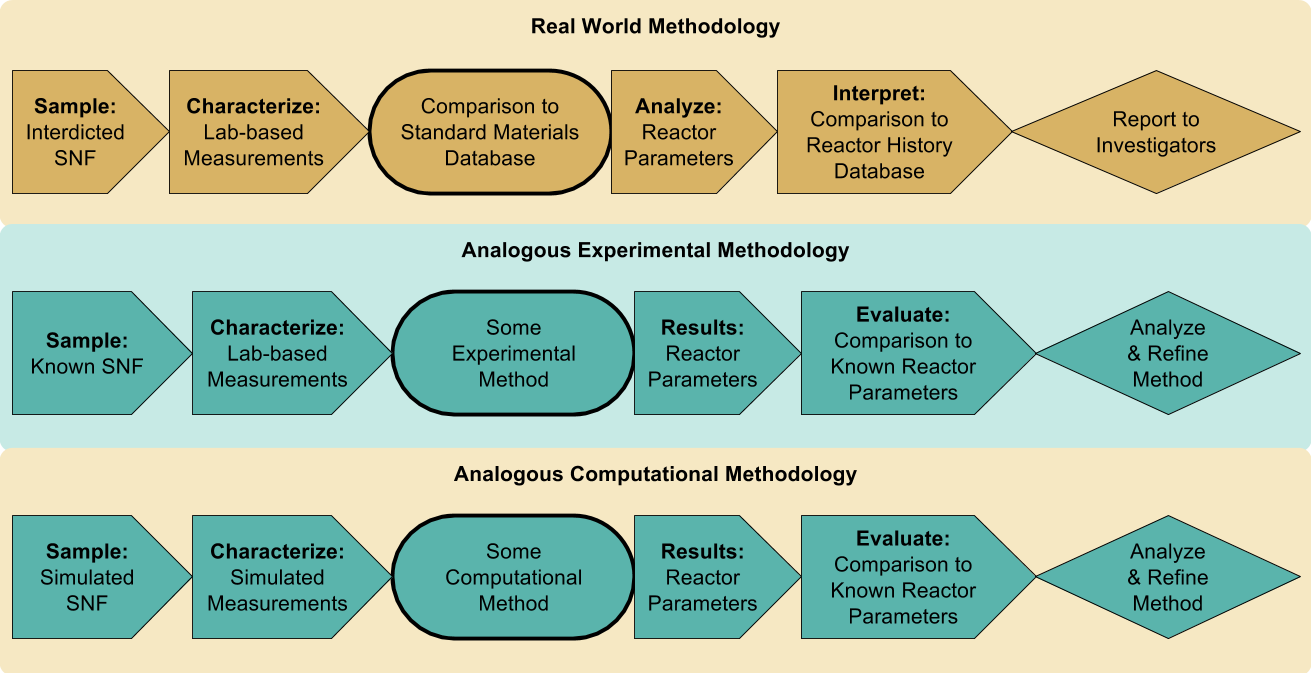
\includegraphics[width=1.1\linewidth]{./chapters/intro/ForensicsWorkflows.png}}
  \caption{Example Forensics Workflows in Real-World Scenario}
  \label{fig:nfworkflow}
\end{figure}

Below the example of a real-world workflow in Figure \ref{fig:nfworkflow} are
analagous experimental workflows, both physical and computational.  
\todo{Fix up diagram to be more aligned with discussion} 
For researchers studying
alternative measurement techniques or a slight difference in the overall
approach, it is necessary to iterate through multiple studies using known
materials to probe sensitivities or other weaknesses in the procedure.

\subsection{Nuclear Forensics as an Inverse Problem}
\label{sec:inverse}

Nuclear forensics is a traditional inverse problem, which has been well
documented in mathematics and many scientific disciplines.  Understanding
inverse problem theory can help systematically define both the solution methods
and their limitations. This section provides an introduction to the topic as
well as its application to nuclear forensics. 

As outlined in a textbook on the formal approach to inverse problem theory
\cite{inverse_theory}, the study of a typical physical system encompasses three
areas:
\begin{enumerate}
  \itemsep-0.75em
  \item \textit{Model parameterization}
  \item \textit{Forward problem:} predict measurement values given model parameters
  \item \textit{Inverse problem:} predict model parameters given measurement values
\end{enumerate}

First, this shows that it is important to consider the parameters that comprise
a model; this is denoted as the \textit{model space}. This is not every
measurable quantity; domain knowledge is necessary to determine the model
space. In the nuclear forensics context for \gls{SNF}, this would consist of,
e.g., several isotopic ratios because they are known to have a relationship
with the reactor parameters that created the fuel of interest.

Second, understanding the physical system also requires an understanding of the
forward problem: predicting how a certain set of model parameters will affect
the resulting measurements. The breadth of these end measurements provides the
\textit{data space}, which are all the conceivable results of a given forward
problem. So for \gls{SNF} this would be, perhaps, the range of isotopic ratios
typical of a commercial reactor. 

Lastly, the inverse problem is statistical in nature: given some solution,
there is a probability that the data measured is caused by some value(s) of a
model parameter. Including measurement uncertainties broadens the linear model
to probability densities of the parameters. The opposite is also true in the
forward case: including parameter uncertainties broadens the forward problem
results to probability densities of the potential measurement values.
\cite{inverse_theory}

In this way, we can define some probability that the answer is correct, given a
set of measurements and their uncertainties. Inverse problem theory states that
this follows the general form of Bayes' theorem, which is commonly expressed as
follows:
\begin{equation}
  \label{eq:bayes}
  P(A|B) = \frac{P(B|A)P(A)}{P(B)}
\end{equation}
where $A$ and $B$ are events, $P(A)$ and $P(B)$ are the probabilities that events
$A$ and $B$ will occur, respectively, $P(B|A)$ is the likelihood that event 
$B$ will occur given a known result for $A$, and $P(A|B)$ is the posterior 
probability that event $A$ will occur given a known result for $B$.

This is can be mapped easily to the inverse physical system problem scenario.
$A$ would represent an occurence of a parameter in the model space, and $B$
would represent the measurement of some value. Thus, $P(A)$ is the probability
of a parameter existing without any knowledge of $B$. This is known as the prior
probability, usually given by some theory about the system. $P(B)$ is the
probability of some measurement existing without any knowledge of $A$. This is
known as the marginal likelihood, which is some homogeneous concept for the
potential measurements that could be made (this only serves to scale to absolute
probabilities and does not affect the relative probabilities). The likelihood,
$P(B|A)$, is the chance that a measurement is observed from a given parameter,
representing the forward problem.  Lastly, the posterior probability is the
chance of some parameter existing given some measurement, representing the
inverse problem solution \cite{inverse_theory, gentle_bayes}.  It may be more
intuitive to consider the conceptual version of Bayes' theorem below.  A
discussion of how these values are obtained takes place in Section
\ref{sec:invcompare}.
\begin{equation}
  \label{eq:bayes_words}
  Posterior = \frac{Likelihood * Prior}{Marginal \ Likelihood} 
\end{equation} 

This framework is helpful for an experiment that intends to compare different
methods for calculating the posterior probability of a system given some
measurements \cite{bayes_compare}.  In the nuclear forensics context of
pre-detonated materials, this would be a a set of probabilities for different
parameters of interest, e.g., reactor type, burnup, cooling time, and
enrichment of some interdicted \gls{SNF}. 
